Bisher waren wir ausschließlich mit deterministischen Signalen befasst. 
Also solchen, welche sich bequem durch eine Funktionsvorschrift $t \mapsto x(t)$ beschreiben lassen.
Doch eigentlich ist dies ein absolut idealisierter Spezialfall, da für gew\"ohnlich alle Signale, die wir verarbeiten, zu mindestens einem Zeitpunkt von einem Messgerät beobachtet wurden.
Somit sind diese notwendigerweise mit Messrauschen behaftet, dessen unangenehme Eigenschaft es ist, zuällig zu sein.
Aus diesem Grund ist es uns nicht m\"oglich, ein gemessenes und digitalisiertes Signal $x[\cdot]$ mittels eines alebraischen Ausdrucks zu beschreiben.
Notwendigerweise wird $x[\cdot]$ zu einer sog. Zufallsgr\"oße, welche wir \q{nur} noch durch deren statistische Eigenschaften beschreiben k\"onnen.
Nicht nur das, auch jede folgende Verarbeitung von $x[\cdot]$, bespielsweise durch ein \gls{lti}-System, wird zu einer Zufallsgr\"oße, deren Eigenschaften u.A. von denen des Messrauschens abhängen.

Weiterhin kann es für gewisse Anwendungen auch absolut ausreichend sein, eigentlich deterministische Signale als zufällig zu modellieren.
Wenn es beispielsweise darum geht, zu bestimmen, ob ein Kommunikationssystem in der Lage ist, Informationen fehlerfrei zu übertragen, dann kann es ausreichend sein, \q{nur} eine Ausfallrate zu bestimmen, oder diese Rate zu begrenzen, anstatt dies für jedes m\"ogliche übertragene Signal zu bestimmen/gewährleisten.

Um diese \q{neue} Sichtweise auf Signale gut verinnerlichen zu k\"onnen, ben\"otigen wir jedoch einige Werkzeuge aus der Wahrscheinlichkeitstheorie, die wir uns nun ansehen werden, wobei wir versuchen, uns nicht mit vielen mathematischen Details aufzuhalten, sondern wollen stattdessen unsere Intuition schärfen.

\subsection{Grundlagen Wahrscheinlichkeitstheorie}\label{sec:random:prbly}

Nehmen wir zunächst einmal an, dass wir einen zufälligen Vorgang betrachten, dessen Ausgang sich in Form einer einzelnen reellen Zahl manifestiert.
Diesen zufälligen Vorgang assoziieren wir mit der Zufallsgr\"oße $X : \Omega \rightarrow \R$, also $\omega \rightarrow X(\omega)$, wobei wir uns vorstellen, dass $\Omega$, beziehungsweise $\omega$, dafür sorgen, dass Zufall ins Spiel kommt. \textit{$\ast$MITHÄNDENWEDEL$\ast$} Wir sind nun daran interessiert, wie die \emph{Verteilung} der Werte $X(\omega)$ charakterisiert werden kann.

Hierzu definieren wir beigeordnet zu $X$ eine Funktion $F_X: \R \rightarrow [0,1]$, welche uns für $x \in \R$ mitteilt, was die Wahrscheinlichkeit für das Ereignis $X \leqslant x$ ist.
Man kann auch sagen/schreiben:
\[
F_X(x) = P(X \leqslant x).
\]
Die Funktion $F$ ist monoton wachsend, da natürlich $P(X \leqslant x_1) \leqslant P(X \leqslant x_2)$, falls $x_1 < x_2$, also auch $F_X(x_1) \leqslant F_X(x_2)$.
Jetzt kann man mit der \emph{Verteilungsfunktion} $F_X$ schon eine Menge anfangen.
Beispielsweise k\"onnen wir damit auch bestimmen, mit welcher Wahrscheinlichkeit das Ereignis $x_1 < X \leqslant x_2$ eintritt, indem wir einfach 
\[
P(x_1 < X \leqslant x_2) = F_X(x_2) - F_X(x_1)
\]
berechnen.

Wir k\"onnen sogar noch einen Schritt weiter gehen, und die Gr\"oße
\[
f^h_X(x) = \frac{F_X(x + h) - F_X(x)}{h}
\]
betrachten.
Man kann es sich so vorstellen, dass wir das Intervall $[x,x+h]$ hernehmen, berechnen, wie \q{viel} von $X$ in $[x,x+h]$ landen kann, und normieren das mit der Intervallbreite $h$.
Im Grunde berechnen wir, wie \q{dicht} die Zufallsgr\"oße zwischen $x$ und $x+h$ ist.
Aus diesem Grund nennt man
\[
f_X(x) = \lim\limits_{h \rightarrow 0} f^h_X(x) = \lim\limits_{h \rightarrow 0} \frac{F_X(x + h) - F_X(x)}{h}
\]
die \emph{Dichte} von $X$.
Natürlich sehen wir, dass der berechnete Grenzwert der sogenannte Differenzenquotient der Verteilungsfunktion $F_x$ ist. Es gilt also $f_X = F^\prime_X$.
Deshalb kann man nun die Verteilungsfunktion auch aus der Dichte gewinnen, indem wir
\[
F_X(x) = \Int{-\infty}{x}{f_X(s)}{s}
\]
auswerten.
Die obigen Betrachtungen gelten freilich nur, wenn die formulierten Grenzwerte auch immer existieren, doch erstens existieren diese meistens und für ein intuitives Verständnis sollte es zunächst genügen.

Weiterhin gilt für reelle Zufallsgrößen $X$, dass diese sich \q{irgendwo} zwischen $-\infty$ und $+\infty$ mit Wahrscheinlichkeit $1$ realisieren muss.
Also gilt
\[
\lim_{x \rightarrow \infty} F_X(x) = 1,
\]
was für die Dichte ergibt, dass
\[
\Int{-\infty}{+\infty}{f_X(s)}{s} = 1.
\]
%
%
\subsubsection{Beispiele}
%
\paragraph{Uniforme Verteilung/Gleichverteilung}
Gegeben zwei reelle Zahlen $a < b$ nennt man eine Zufallsgröße $X$ verteilt nach $\Unif(a,b)$, wenn die Dichte $f_X$ gegeben ist durch
\[
f_X(x) = \begin{cases}
    0, \Text{falls} x<a, \\
    1/(b-a), \Text{falls} a \leqslant x < b \\
    0, \Text{falls} b \leqslant x.
\end{cases} = 
    \frac 1{b-a} \Rect\left(\frac{x-(b+a)/2}{b-a}\right)
\]
Der Name dieser Verteilung ergibt sich daraus, dass intuitiv alle Intervalle, die im Intervall $[a,b]$ liegen mit einr Wahrscheinlichkeit proportional zu ihrer \q{Länge} von $X$ \q{getroffen} werden.
Man schreibt auch oft $X \sim \Unif(a,b)$.
%
\paragraph{Normalverteilung}
Gegeben zwei Parameter $\mu \in \R$ und $\sigma^2 \in \R^+$, so nennt man eine Zufallsgröße $X$ normalverteilt mit Erwartungswert $\mu$ und Varianz $\sigma^2$, falls deren Dichte $f_X$
\[
f_X(x) = \frac{1}{\sqrt{2 \pi \sigma^2}} \exp\left(-\frac{(x - \mu)^2}{2 \sigma^2}\right)
\]
erfüllt.
Die Normalverteilungist eine sehr wichtige Verteilung, weil aus Gründen die meisten Messwerte einer Normalverteilung mit Erwartungswert $\mu$ und einer gewissen Varianz $\sigma^2$ folgen.
Je größer $\sigma^2$, desto stärker ist die Streuung der gemessenen Werte um den Erwartungswert $\mu$.
Man schreibt auch $X \sim \mathcal{N}(\mu, \sigma^2)$.
Es sind zwei Beispiele in \Cref{py:random:normal1} zusammen mit der Berechnung der Dichte via \texttt{scipy} dargestellt.
Auch hier ist es wieder ratsam, keine eigenen Implementierungen solcher Standardfunktionen zu nutzen und stattdessen auf Funktionen aus getesteten Paketen zurück zu greifen.
\begin{listing}[ht]
    \noindent
    \begin{minipage}{0.51\textwidth}
        \strut\vspace*{-\baselineskip}\newline
        \inputminted[firstline=3, lastline=10]{python3}{code/random/normal1.py}
    \end{minipage}%
    \begin{minipage}{0.48\textwidth}
        \strut\vspace*{-\baselineskip}\newline
        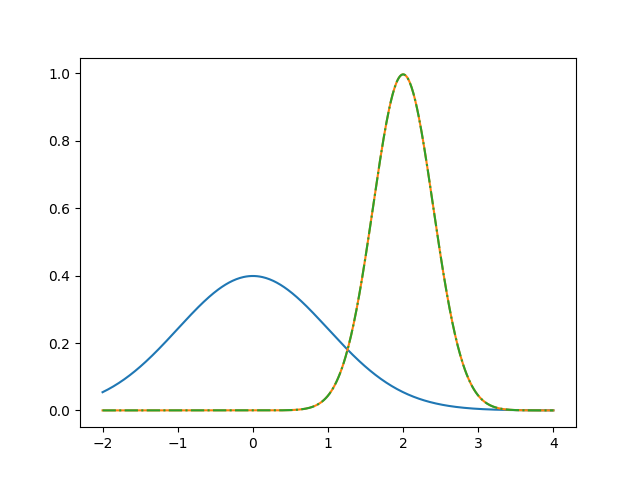
\includegraphics[width=\textwidth]{code/random/normal1.png}
    \end{minipage}
    \codecaption{dsv/code/random/normal1.py}{Visualisierung der Dichte der Normalverteilung für verschiedene Parameter}\label{py:random:normal1}
\end{listing}
%
%
\paragraph{Exponentialverteilung}
Gegeben eine Intensität $\lambda > 0$, so folgt eine Zufallsgröße $X$ einer Exponentialverteilung $\Exp(\lambda)$, falls die Dichte $f_X$ die Form 
\[
f_X(x) = \begin{cases}
    \lambda \exp(-\lambda x), \Text{für} x \geqslant
    0, \\
    0 \Text{sonst}
\end{cases}
\]
besitzt.
Auch eine wichige Verteilung, die beispielsweise die Lebensdauer von irgendwelchen Bauteilen modelliert, oder auch die Wartezeit zwischen zwei Anrufen bei einer Servicehotline. 
Je kleiner $\lambda$, desto höher die Intensität, also desto kürzer die Wartezeit.
%
%
\subsubsection{Erwartungswert, Varianz, Kovarianz}

Will man eine Zufallsgröße auf einige wenige Kennzahlen herunterbrechen, die in der Praxis auch relevant sein könnten, so bieten sich sogenannte Momente deren Verteilung an.
%
%
\paragraph{Erwartungswert}
Interessiert man sich für den Wert, der sich \q{im Mittel} bei einer Verteilung $X$ ergibt, so berechnet man den Erwartungswert $\E(X)$ definiert durch
\begin{equation}\label{eq:random:mean}
    \E(X) = \Int{-\infty}{+\infty}{x f_X(x)}{x}.
\end{equation}
Wenn $f_X$ einer physikalischen Dichteverteilung im Raum entspräche, so würde $\E(X)$ genau den Masseschwerpunkt dieser Verteilung darstellen.
Ist beispielsweise $X \sim \Unif(a,b)$, so gilt $\E(X) = (a+b)/2$ und falls $X \sim \mathcal{N}(\mu, \sigma^2)$, so gilt $\E(X) = \mu$.
%
%
\paragraph{Varianz}
%
Basierend auf dem Erwartungswert, können wir auch die erwartete Streuung einer Zufallsgröße um $\E(X)$ herum betrachten, also
%
\begin{equation}\label{eq:random:var}
\Var(X) 
    = \E((X - \E(X))^2) 
    = \Int{-\infty}{+\infty}{(x-\E(X))^2 f_X(x)}{x}
    = \E(X^2) - \E(X)^2.
\end{equation}
%
Die Interpretation ist, dass $\Var(X)$ die mittlere quadratische Abweichung einer Zufallsgröße von ihrem Erwartungswert beschreibt.
Es ist anzumerken, dass es Verteilungen gibt, für welche $\E$ und $\Var$ nicht existieren müssen, weil die jeweiligen Integrale in \eqref{eq:random:mean} und \eqref{eq:random:var} nicht endlich sind.

Beispielsweise gilt im Falle von $X \sim \Unif(a,b)$, dass $\Var(X) = (b-a)^2/12$ und im Falle von $X \sim \mathcal{N}(\mu, \sigma^2)$, dass $\Var(X) = \sigma^2$.

\subsection{Zufällige Signale}

% - Stochastische Prozesse: definition, zwei sichtweisen (per pfad, folge von verteilungen)
% - stationaere prozesse/signale
% - Wiener-Chintschin-Theorem

\subsection{Parameterschätzung}\label{sec:random:paramest}

\subsection{Quantisierung}\label{sec:random:quanti}

% - \cite{widrow2008quantization}
% - area sampling (geoemetrisch)
% - charakteristische funktion: value at 0, conj sym, 
% - areasampling: analytisch in value domain, in frequ domain
% - reconstruction der PDF aus der quantisierten PDF
% - PQN Model